% !TEX root = ../dissertation.tex

\chapter{Sancho Overview}
\label{chapter:sancho_overview}

A more up to date and detailed overview of the Sancho project is given in this chapter

\section{The overall architecture}

Sancho is based on the ggp-base framework, which includes an interpreter for GDL descriptions, a basic propositional network constructor among a few other things. Some of these components are heavily modified in Sancho.
It spawns many different threads but there are only 3 important types:

\begin{itemize}
	\item 1 HTTP server thread: Responsible for network communication with the game manager.
	\item 1 MCTS structure control thread: Handles all MCTS steps except simulation. It's the only thread that can modify the MCTS graph.
	\item N Playout threads: These threads handle simulations (random playouts).    
\end{itemize}

Some other threads are spawned by the ggp-framework itself, like the GUI thread, but aren't important to Sancho's performance.

\begin{figure}[h]
	\centering
	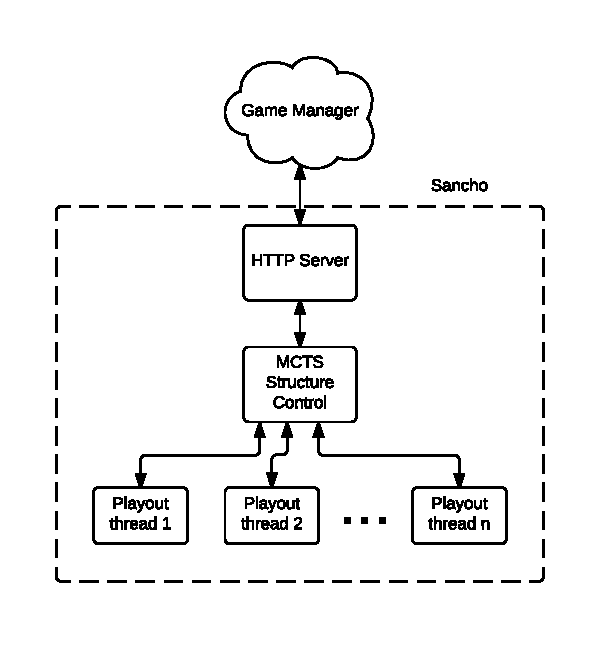
\includegraphics[width=0.6\textwidth]{images/Sancho_overview.pdf}
	\caption{Sancho threading overview}
	\label{fig:sancho_overview}
\end{figure}


\begin{figure}[h]
	\centering
	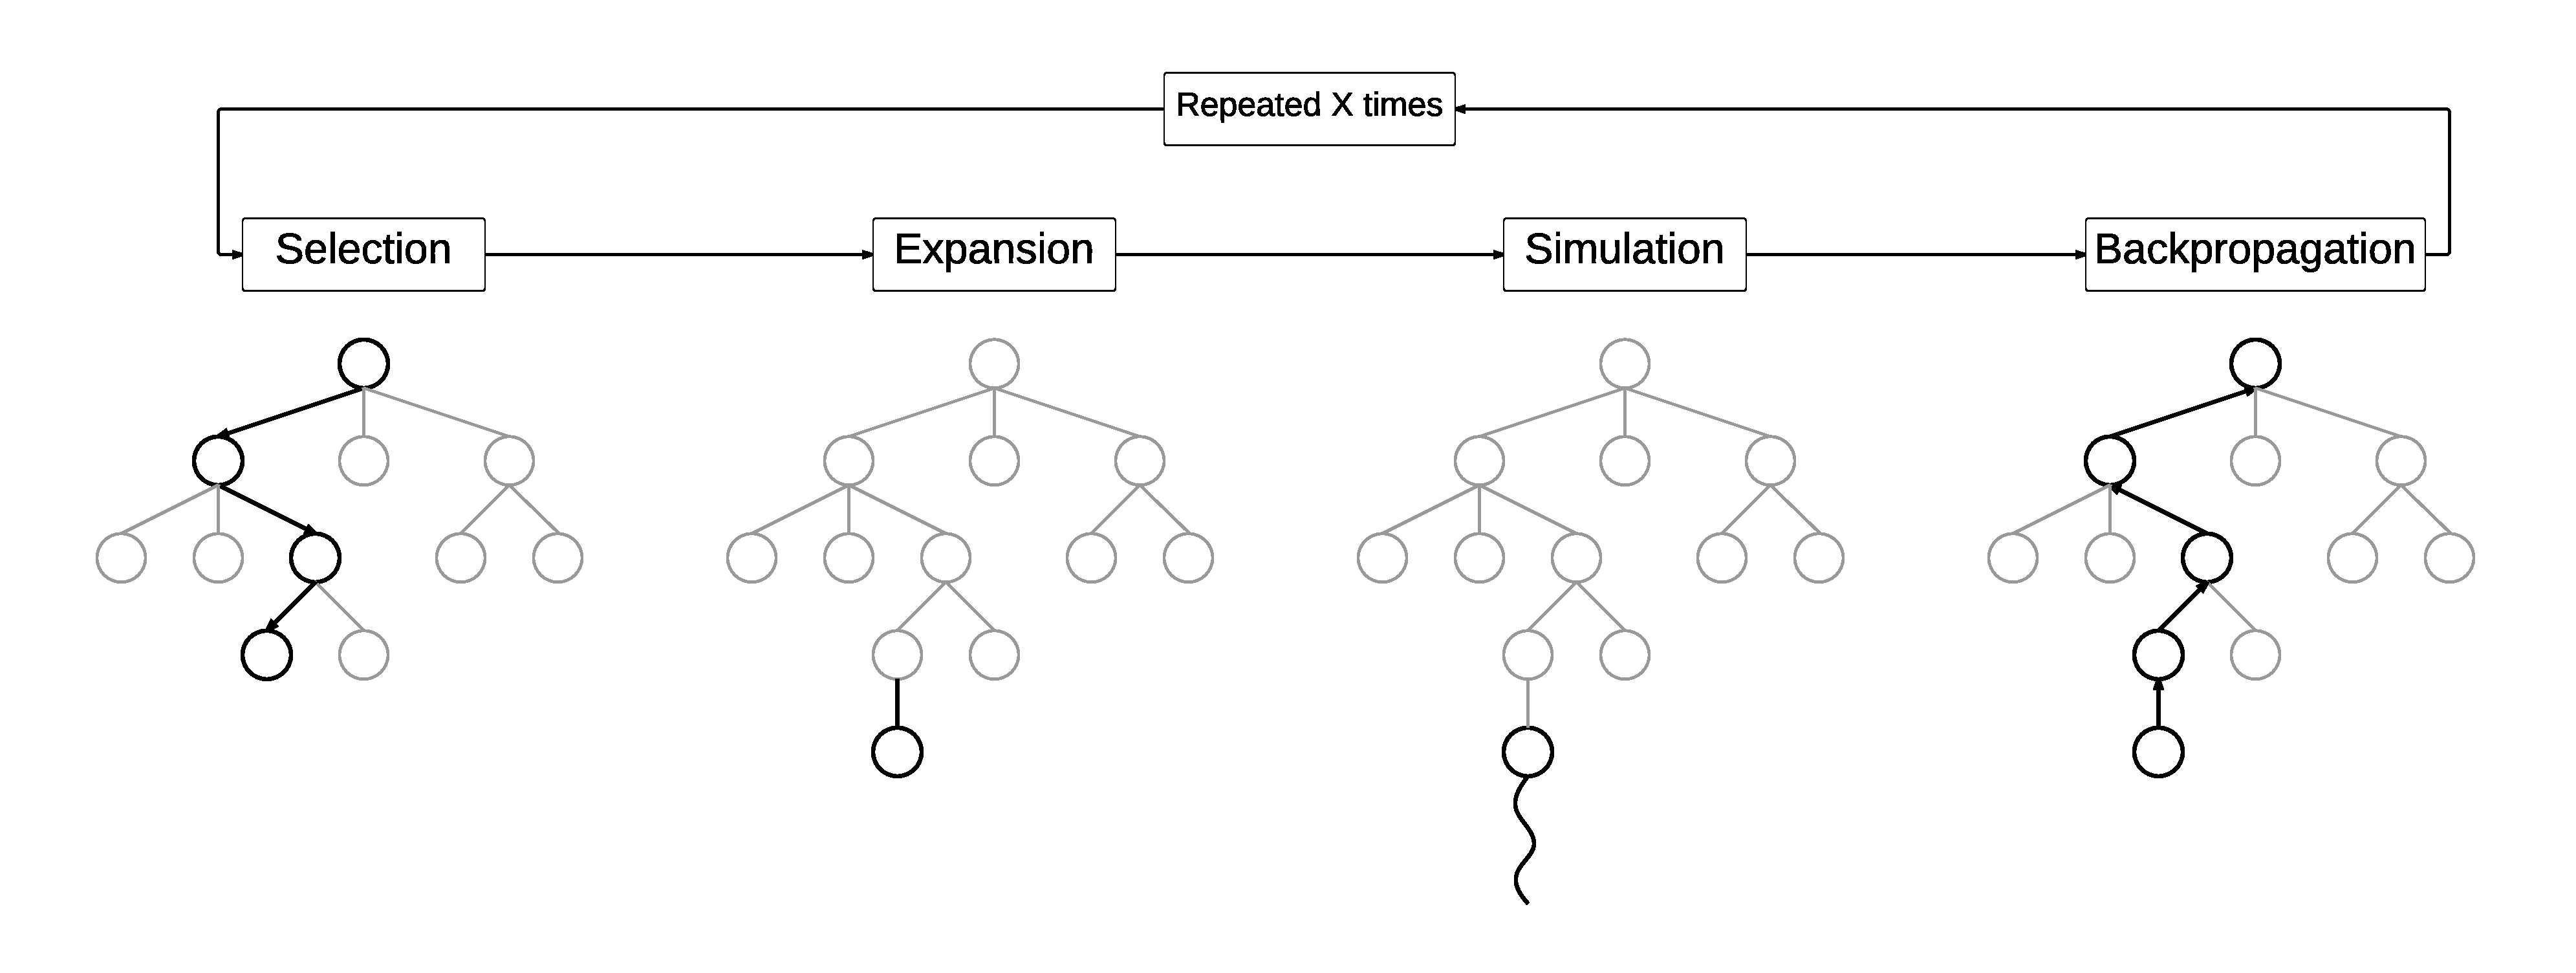
\includegraphics[width=\textwidth]{images/MCTS.pdf}
%	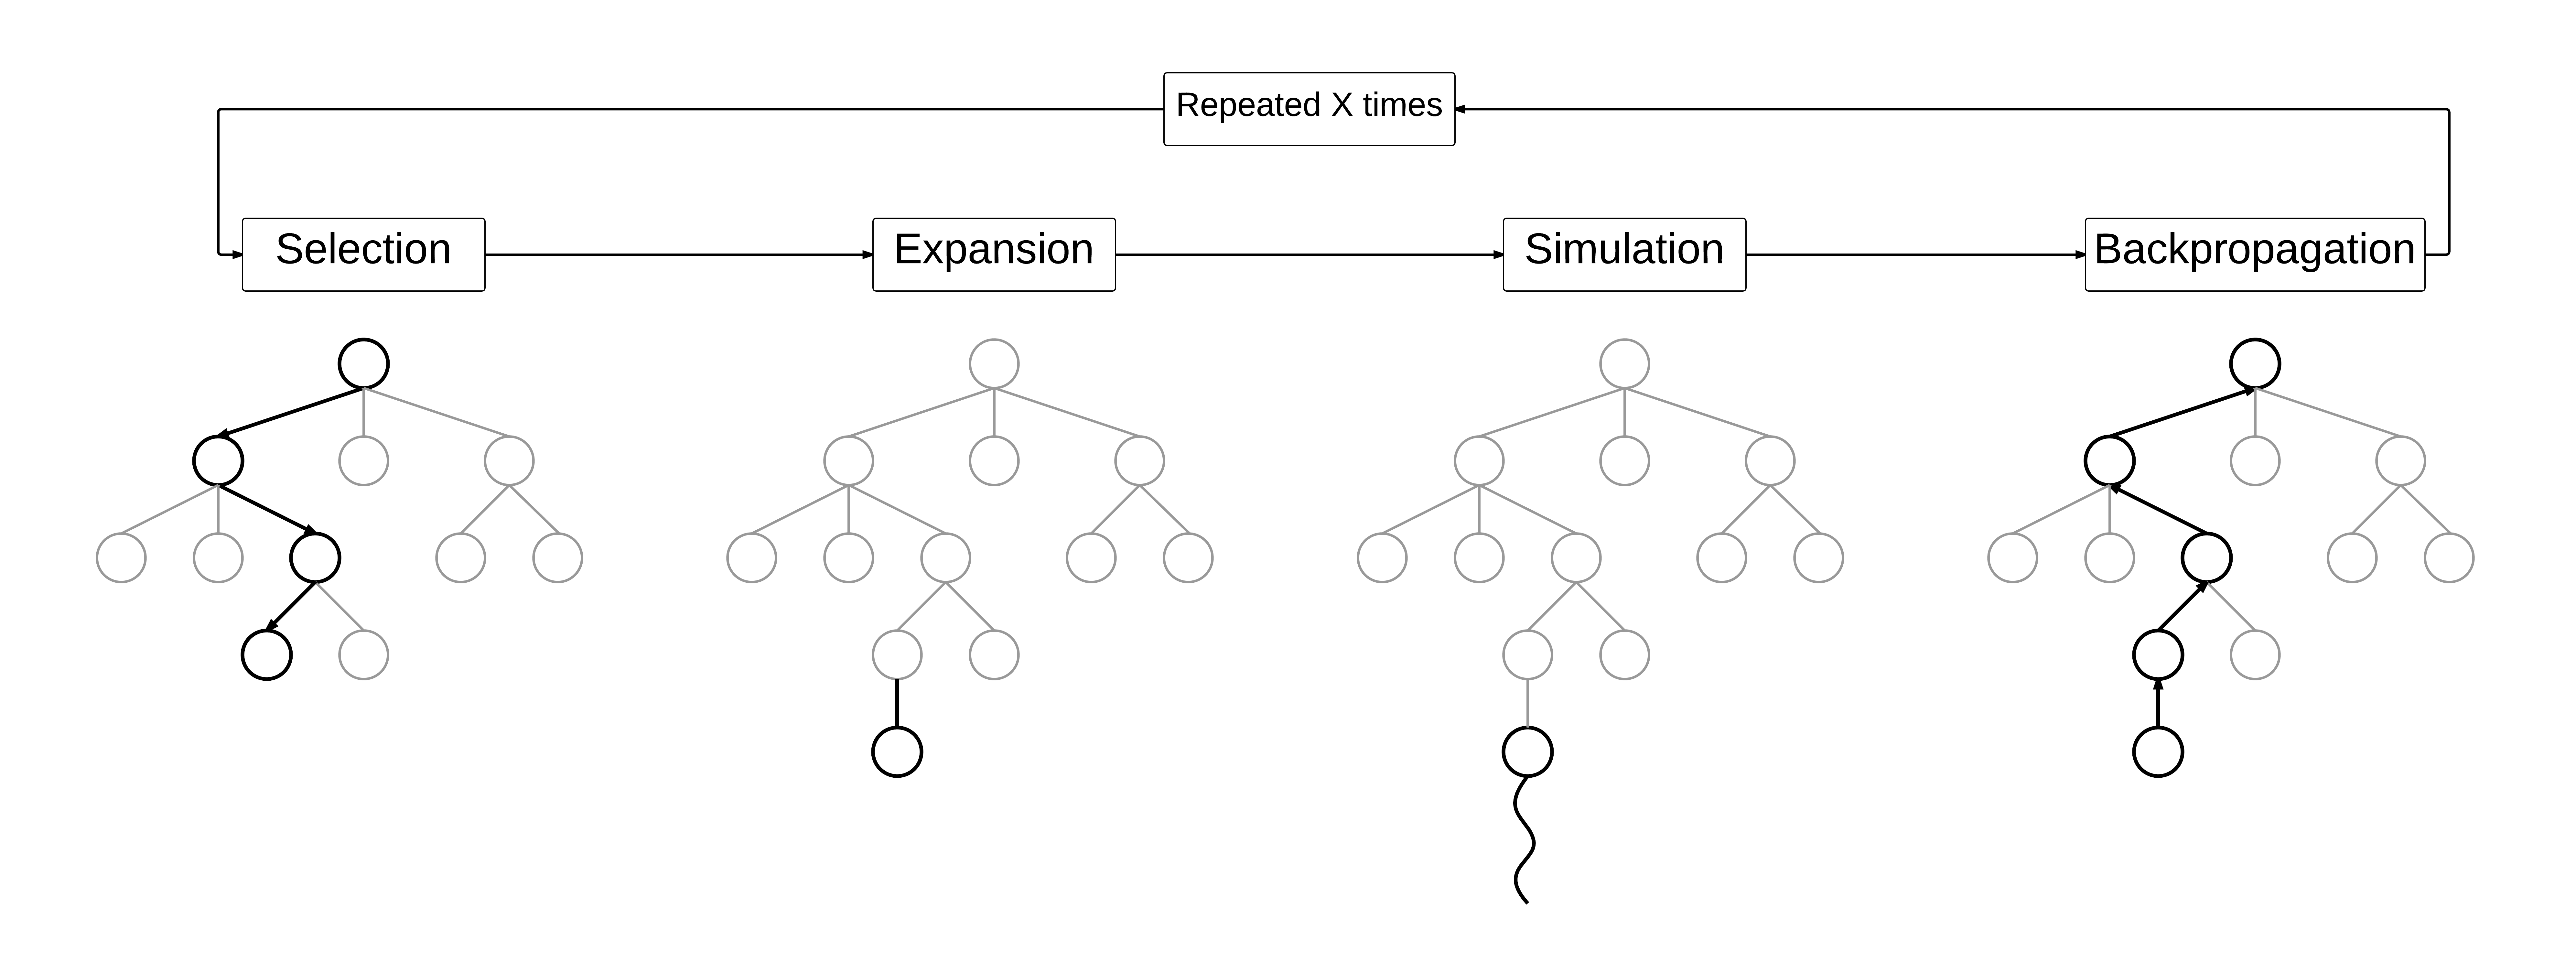
\includegraphics[width=\textwidth]{images/MCTS.png}
	\caption{MCTS steps}
	\label{fig:mcts steps}
\end{figure}

\section{MCTS data structure}
MCTS is usually done on a tree structure but Sancho uses a Directed Graph to represent the game states and transitions, allowing for each state to be represented only once, regardless of the path taken to reach it.
This has two main advantages: the values for each state can be drastically more accurate by averaging the scores from different paths and it can also save on memory.
The main drawback is making back-propagation more complicated to implement.


\section{Meta-Gaming}
Before a match actually starts players have a time period to prepare themselves, lasting about 3 to 4 times the length of a normal turn. This is called the Meta-Gaming time and can be used not just for initialization but also to do game analysis and other optimizations.

Sancho does the following types of analysis during Meta-Gaming: 
\begin{itemize}
	\item Static dependency analysis: the distances between propositions are evaluated (how many transitions are between proposition A and proposition B). This can be useful to create "close-to-goal" heuristic or to choose the UCT's exploration coefficient. 
	
	\item Factorization: Identifying composite games or similar factorization opportunities. This is usually done by identifying a goal that is OR condition of other "semi-goals" which can thus be factored into multiple Propositional Networks, each with one of these "semi-goals".	 
	
	\item Statistical analysis, described in \ref{sssec:statistics_gathering}
\end{itemize}

\subsection{Statistics gathering}
\label{sssec:statistics_gathering}
A large part of Sancho's Meta-gaming time is used to gather statistics about the game. This is done by simulating many instances of the game, usually completely random or with few improvements, and gathering data about, among others:

\begin{itemize}
	\item Distribution of game length
	\item Average branching factor
	\item Presence of simultaneous moves
	\item How effective greedy playouts are and how costly
	\item Correlation of candidate heuristic signals and outcomes
	\item Are piece heuristics useful
	\item How fast are simulations (to set the sample size of each simulation step)
\end{itemize}

\section{Heuristics}
Sancho uses heuristics to improve the convergence time of MCTS. They are used when first expanding a node, to initialize it with a meaningful score. For example, heuristics that might reflect piece counts, piece captures or numeric quantities can be very useful in many games. Nodes keep track of how many simulations have been done so that score confidence can be taken into account. 

Heuristics should be dynamically generated for the game being played so that the player can adapt to any game, although pre-made heuristics can also be used as long as there is a process to disable them when not suitable.


\subsection{Generation of candidate Heuristics}
Static analysis is used to generate \textit{possible} heuristics, with no regard for whether they are actually useful at all, for now. At this point the requirements are that they should be calculable given a state or move (moves are bit hard to define, this will be touched in more detail later) and should cheap to compute.


\subsection{Crystalization of Heuristics}
After generating heuristics several game thousands of random game simulations are done to gather statistics about the game and on the performance of candidate heuristics, so they can be weighted or completely disabled based on the results. They are then used  on the expansion phase of MCTS to initialize the node with a weighted average heuristic value.


\subsection{Move Heuristics}
Move heuristics are harder to derive since in most games moves aren't intrinsically good or bad, without the context of state. 
Similarity of states isn't well defined, Sancho's definition is that a small number of difference in propositions values means similarity. 
It uses locality sensitive hash techniques are used to create \textit{buckets} of similar states.
The move heuristic will then have a value for each \textit{bucket} and when doing node expansion the heuristic value for the state's bucket is evaluated.


\section{Propositional Networks Implementation}

Propositional Networks (PropNets) are used in Sancho as a faster way of computing state transitions than interpreting GDL. An example was given in  figure \ref{fig:propnets example}.
GDL can be translated into a PropNet representation since both are first order logic, GGP-base includes a GDL to PropNet converter which Sancho builds on to improve performance.


\subsection{Data Representaion}
\noindent PropNets are represented in a way that enables cheap state updates and queries:
\begin{itemize}
	\item All components store their own current state to avoid calculating state on queries. By caching the states, calculation only has to happen when a base proposition changes value.
	
	\item Logic components can have more than 2 inputs, to avoid having to represent a 5-input AND gate with 4 2-input AND gates that take up more memory and increase time complexity of propagation
	
	\item AND and OR gates store their state as an integer with a value equal to the number of inputs set to True, so that whenever one of the inputs changes, all that has to be done to calculate the new output is to increment or decrement the integer and do a simple if statement. (This is actually done a bit more efficiently but the idea is very similar)
	
	\item PropNet state (values of components) and structure (component type and connections) are stored separately, so that multi-threading is possible: the PropNet structure is shared and read-only and each thread stores it's own version of PropNet state, so that no blocking is needed. These threads can then be used to calculate different state-transitions in parallel. More details about how this is stored are given below.
\end{itemize}

The PropNet structure itself (what components exist and what they're connected to) is stored in two fixed length arrays, as can be seen in \ref{fig:propnet_structure}.
PropNet states are also stored in fixed length arrays, where each entry is the value of a base proposition of the net.

Note: During the creation and optimization process of the propnet Sancho actually uses more dynamic and high-level data structures from Java's collections. When the final topology is reached the conversion to these low-level/high-performance data structures is done.
	
\begin{figure}[h]
	\centering
	\includegraphics[width=0.75\textwidth]{images/PropNet_Structure.pdf}
	\caption{Propositional Network structure}
	\label{fig:propnet_structure}
\end{figure}

\subsection{Implementation optimizations}
After the initial GDL to PropNet translation is done Sancho tries several methods of improving the performance of the network:
\begin{itemize}
	\item All constants are represented by only 2 components (one for \textit{True} and one for \textit{False}) instead of spawning their own.	
	
	\item Several techniques are used to try to reduce the number of components, like doing associative, distributive and DeMorgan's transformations and removal of redundant components (like two NOT gates in series) and duplicate components. 

	\item Moving goal score calculation to a separate network since it's only relevant on terminal states, so it's ok to calculate it's values from scratch when needed (by querying the current values of the main network) because it's rarely needed.
	
	\item Whenever a component changes value it forces a recalculation on all components that it outputs to,  initiating a forward-propagated update of the PropNet.
	It's actually a differential forward propagation, since components only propagate updates if their own outputs change
	
	\item When possible, factor the network into multiple independent sub-networks. This happens with compound games (n independent games glued together) and is a big win in performance because it reduces the branching factor to a+b instead of a*b, where a is the branching factor for one game and b for the second (there can of course be more than 2)
	
	\item Moving control logic (like the logic that calculates whose turn it is) out of the PropNet and converting it into functions like counters
	
\end{itemize}

A note on moving control logic out of the PropNet: It can also allow for game approximation, a technique where the player deliberately simplifies the goal value calculation in a lossy way, effectively playing a different but simpler and similar game.

\iffalse
\begin{itemize}
	\item Game is win/draw/loss based on who holds the biggest number of a certain set of base propositions
	
	\item Game is win/draw/loss 
	
	\item Goal value is based on the number of some set of base propositions that are set to true
	
	\item Like any of the above but where the count is represented by a succession of counting propositions
\end{itemize}
\fi

\section{Multi-Threading}
Sancho, being based on GGP-base, spawns several threads from the framework itself that aren't relevant to it's performance, like the HTTP server or the GUI.
An overview of the relevant thread structure can be seen in figure \ref{fig:sancho_overview}. There are only 2 important types of threads: the MCTS structure control thread and the Playout threads.

The MCTS structure control is in charge of 3 of the 4 MCTS steps (figure \ref{fig:mcts steps}), all except simulation, which is the task of the playout threads.
Essentially the MCTS thread traverses the graph selecting nodes based on a version of UCT (\ref{UCT}), expanding them (the score is initialized based on the active heuristics) and adding them to the simulation queue. After it gets the results from the playout threads the new information is back-propagated through the current move sequence.

Playout threads get tasks from the simulation queue and use the PropNet structure to make playout simulations. In Sancho these playouts can either be random or greedy. Greedy playouts perform 1-level deep lookahead and choose immediate wins and avoid immediate losses, they can be very useful in some games but are also quite expensive so they are only used if the Meta-Gaming analysis concludes that they are a net benefit for the current game. Each of these threads keeps their own version of the game state to avoid the need for locking. Playout threads are actually much faster than the MCTS thread so they usually do multiple playouts from the same node and return the average result.


\section{Search optimizations}

\section{Latch Detection}
Latches are propositions that once set can never become unset, i.e., when they switch from \textit{False} to \textit{True} they can never change back (or vice-versa). Identifying propositions like this can be very useful in terms of limiting the search space (if it limits the obtainable goals) or in reducing the computational effort of calculating state transitions, since their value can simply be cached and never recalculated.

Sancho does latch detection by PropNet analysis and currently only detects simple cases where a proposition is fed back into itself, making it's next value dependent on the current value, in one of the following ways:

\begin{itemize}
	\item $A' \leftarrow A$ or $<other conditions>$ (positive latch)
	\item $A' \leftarrow \bar A$ and $<other conditions>$ (negative latch)
	\item $B \leftarrow A$ or $<other conditions>$ (positive latch if A is positively latched)
	\item $B \leftarrow A$ and $<other conditions>$ (negative latch if A is negatively latched)
\end{itemize}


\subsection{Goal Latches}
Detecting goal latches can lead to further optimizations than simply caching results, since they can give additional information like the new maximum or minimum attainable scores and can thus severely impact the way search is done from then on. It can also be used in conjunction with an heuristic that tries to raise the minimum attainable score and avoids lowering the maximum.
Latch detection in the way Sancho implements is very cheap and be done at startup, allowing this heuristic to be used on the meta-gaming playouts.

\iffalse
\section{Local Search}
Certain games or game features can have a sort of locality, where certain moves only affect some other features of the game within a certain "distance". This is easily visualized in many board games but can happen in more abstract forms. This can possibly allow the player to divide the the game into sections of influence (that can still affect each other, unlike factorized games).

A distance heuristic can be statistically determined and then moves in a sphere of influence can be calculated based on this. 
\fi


\section{1-player games (puzzles) solving}

When Sancho plays single player games, or puzzles, it tries to use different methods to decide its strategy, since it can control the whole game and thus only needs to find a single path to it's target state (the state that finishes the game with the best possible score).
First an attempt at identifying a target state and back-tracing to the root to find the path. This is often impractical because a game might have many target states, most of them unreachable from the starting game state (sudoku, for example) or most paths might simply be too long.

If an admissible path-finding heuristic (one that never over-estimates the real cost of reaching the goal) can be found, A* can be used to attempt finding the optimal path to a target state. The heuristic used by Sancho for A* is Hamming distance (the distance between states is computed as the number of different proposition values).
The factorization of control logic out of the main PropNet can really help performance when using path-finding algorithms.

